%  <-- ezzel lesznek jelölve a kommentek,
%a legtöbb dolgot jobb békénhagyni úgy ahogy van, általában csak {} közé vagy \section{} alá kell írni majd
%az ITKproc miatt nem kell megformáznod a szöveget tehát ezt mindenképpen hagyjátok a itt, valamint mindig legyen a dokumentum mappájában, hogy elérje a fordító
\documentclass[10pt, conference,a4paper]{ITKproc}

\usepackage[utf8]{inputenc}
\usepackage{graphicx}
\usepackage{gensymb}
\graphicspath{ {images/} }
% correct bad hyphenation here

\hyphenation{pre-sence vi-su-alized si-mu-la-tions mo-le-cu-lar se-ve-ral cha-rac-te-ris-tic CoNSEnsX}


\begin{document}
% ide a {} közé írd a jegyzőkönyv címét
\title{GPS mérési jegyzőkönyv}
% ezek gondolom egyértelműek, itt is mindig csak a {} szerkesszétek, valamint használhattok \\ sortöréshez, pl dátum hozzáírás stb
\author{\IEEEauthorblockN{Mátyás Antal}
\IEEEauthorblockA{(Supervisor: Attila Tihanyi)\\
Pázmány Péter Catholic University, Faculty of Information Technology and Bionics\\
50/a Pr\'ater street, 1083 Budapest, Hungary\\
\texttt{antal.matyas.gergely@hallgato.ppke.hu}}
}


\maketitle

\begin{abstract}
A mérés célja volt ismerkedni a műholdas helymeghatározó rendszer elméletével és működésével. A felkészülés során tanulmányoztuk a GPS és GLONASS rendszerek működését, a GPS-es helymeghatározás módszereit, valamint a VisualGPS program kezelését. 
\end{abstract}

\IEEEpeerreviewmaketitle
% innentől kezdve jönnek a feladatok
% \section{} Ezzel hozunk létre fejezetet, a {} közé pedig bármi írhatunk, általában úgyis "Feladat" és "összefoglalás"-t fogunk,
% a fejezetek alapjáraton számozódnak római számokkal tehát azt nem szükséges beleírni, 
% ha alfejezeteket akarunk létrehozni akkor \subsection{} subsubsection{} stb- vel tegyük
%példa:
\section{Mérendő objektumok}

A mérés során részt vettünk a bejáráson, mely során folyamatosan méréseket végeztünk egy GPS vevő és egy számítógép segítségével. A mérési eredményeket a számítógépen a VisualGPS program által generált log fileban, valamint a kézzel írt jegyzőkönyvben tároltuk.  

\section{Útvonal}
Az első feladat a mérés során a számítógép által generált log file vizsgálata volt. A VisualGPS program a file olvasása után a következő útvonalat rajzolta ki:

\begin{figure}[h]
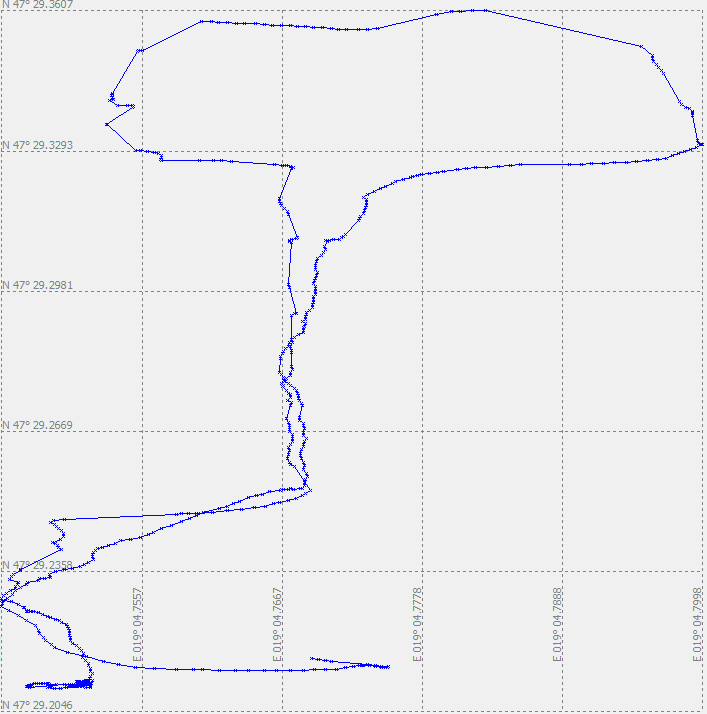
\includegraphics[scale=0.4]{utvonal_visGPS}
\centering

\end{figure}


Ugyanez az útvonal található a jobb oldalon, Google Maps-ben bejelölve az alábbi ábrán látható. A piros jelölés a két pont, melyeket elemeztem. 


\begin{figure}[h]
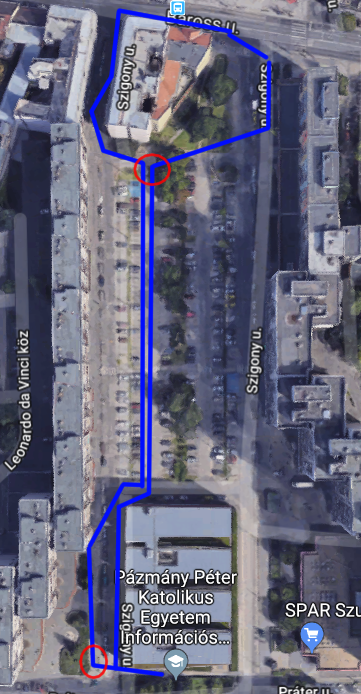
\includegraphics[scale=0.4]{utvonal_googlemaps}
\centering
\end{figure}



\section{Saját pont NMEA kód}
A kapott log file-ban a mérés során készített listában szereplő időpont alapján megkerestem a saját vizsgálandó pontomat, melyet a mérésen 'zebra' névvel jelöltünk. A program az adott időpontban e sort rögzítette:
\\ \\
\$GPGGA,103412.4,4729.21002,N,01904.75113,E,\\1,06,1.3,103.1,M,42.0,M,,*58\\
\\
Melyből kiolvasható, hogy a mérés GPS idő szerint 10:34:12.4 időpontban történt, északi szélesség 47\degree 29.21002', valamint keleti hosszúság 19\degree 4.75113' koordinátán. GPS fix pozícióban. A GPS műszer az adott időpontban 6 műholdat látott, valamint 103 m-es tengerszint feletti magasságban helyezkedett el. 
\section{Koordináták számítása}
Az NMEA kódból kiolvasott koordináták tehát: \\
Ész. 47\degree 29.21002' \\
Kh. 19\degree 4.75113' \\
Mivel 1 szögmásodperc = 1 szögperc 1/60-ad részével: \\
0.21002' =  12.6012''\\
0.75113' =  45.0678''\\
Tehát a saját pontom koordinátái szögfok, szögperc, szögmásodperc formátumban a következők: \\
Ész. 47\degree 29' 12.6012'' \\
Kh. 19\degree 4' 45.0678'' \\
\section{Azimuth térkép}
Az adott mérési pontban a VisualGPS program az alábbi azimuth térképet rajzolta ki:

\begin{figure}[h]
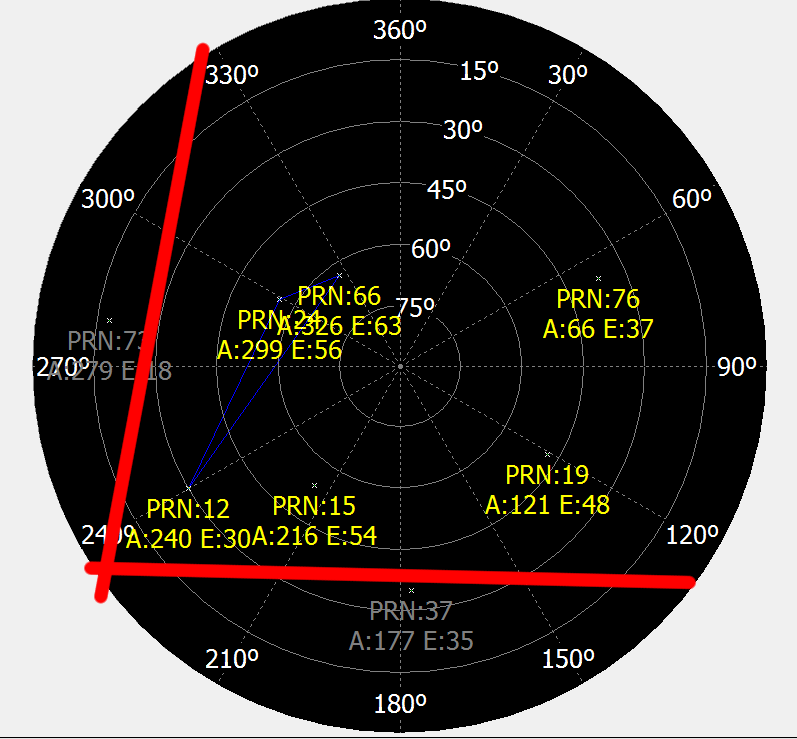
\includegraphics[scale=0.3]{azimuth_sajat_r}
\centering
\end{figure}
A térképen bejelölem az adott pontban lehetséges tereptárgyak elhelyezkedését, melyek ezesetben az utcát határoló magasabb épületek voltak. A mérés pontosságát csökkentheti, hogy kevesebb műhold áll rendelkezésünkre a környezetünkben lévő tereptárgyak árnyékolása miatt. 

Az ábrán továbbá látható az NMEA kódból már kiolvasott 6 műhold, melyek nevét és relatív elhelyezkedését az alábbi táblázat szemlélteti: 




\begin{table}[ht!]
\renewcommand{\arraystretch}{1.3}
\caption{Saját pont műholdjai}
\centering
\begin{tabular}{c||c||c}
\hline
\bfseries Név & \bfseries Irány & \bfseries Látószög\\
\hline\hline
 PRN 24 & 299\degree & 56\degree \\
\hline
  PRN 66 & 326\degree & 63\degree \\
\hline
PRN 76 & 66\degree & 37\degree \\
\hline
PRN 19 & 121\degree & 48\degree \\
\hline
PRN 12 & 240\degree & 30\degree \\
\hline
PRN 15 & 216\degree & 53\degree \\
\hline
\end{tabular}
\end{table}


\section{Szögmásodperc számítása}
A következő feladat volt kiszámítani azt a távolságot, amelyet egy szögmásodperc eltérés jelentett. A számításokat elvégeztük a saját pontunkra, valamint a (0 , 0) pontra is.  
\subsection{Saját mérési pontban}
Saját mérési pontunk szélessége: $47\degree 29.21002', azaz 47 + (29.21002/60) = 47.486833667\degree \approx 47.5\degree$. \\
A $sin(90\degree - 47.5\degree) = \frac{R_{korlemez}}{R_{Fold}})$egyenlet alapján, felhasználva, hogy a Föld sugara az egyenlítőnél 6378.137 km, R = 4326 km, így a kerület $2*R*\pi$ = 27167 km, tehát \\
1\degree = 75.45 km \\ 1' = 1.257 km \\
1'' = 0.021 km. 
\subsection{(0 , 0) pontban}
A Föld kerülete 40.075 km, ezt 360\degree -kal elosztva: \\
1\degree = 111.32 km \\ 1' = 1.85 km \\
1'' = 0.31 km. 
\section{Másik mérési pont}
\subsection{Log file és Azimuth térkép}
Feladat volt továbbá a 'parkoló vége' pont vizsgálata, mely az egyetem mögötti parkolótér végén található 'tűzfal' mellett helyezkedett el. A VisualGPS program által generált log file-ból az adott időpontban a következő sort olvashattuk ki: \\ \\
\$GPGGA,105014.6,4729.32384,N,01904.77738,E,\\1,11,0.7,102.9,M,42.0,M,,*56
\\ \\
Jelentése: A mérés GPS idő szerint 10:50:14.6 időpontban történt északi szélesség 47\degree 29.32384' és keleti hosszúság 19\degree 4.77738' koordinátákon. GPS fix pozícióban. A GPS műszer az adott időpontban 11 műholdat látott, valamint 102 m-es tengerszint feletti magasságban helyezkedett el. \\
A pontban az Azimuth térkép a következő képet mutatta: \\
\begin{figure}[h]
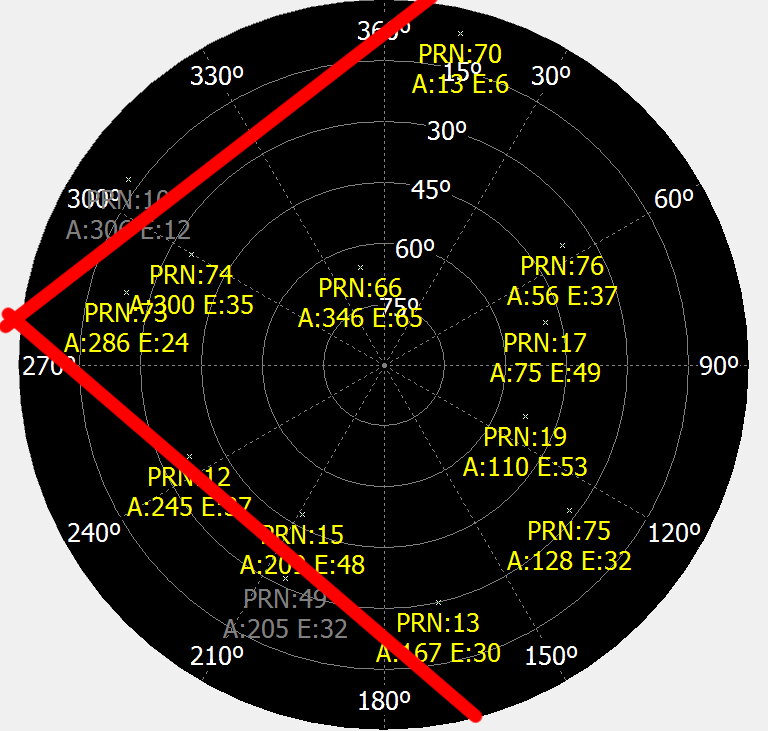
\includegraphics[scale=0.3]{azimuth_kozos_r}
\centering
\end{figure}
A térképen bejelölem az adott pontban lehetséges tereptárgyak elhelyezkedését, melyek ezesetben a parkoló végén álló magas ház, valamint az egyik a parkoló nyugati oldalán található társasház voltak. 
\\
Az ábrán továbbá látható az NMEA kódból már kiolvasott 11 műhold, melyek nevét és relatív elhelyezkedését az alábbi táblázat szemlélteti: 

\begin{table}[ht!]
\renewcommand{\arraystretch}{1.3}
\caption{Saját pont műholdjai}
\centering
\begin{tabular}{c||c||c}
\hline
\bfseries Név & \bfseries Irány & \bfseries Látószög\\
\hline\hline
 PRN 70 & 13\degree & 6\degree \\
\hline
  PRN 74 & 300\degree & 35\degree \\
\hline
PRN 73 & 286\degree & 24\degree \\
\hline
PRN 66 & 346\degree & 65\degree \\
\hline
PRN 76 & 56\degree & 37\degree \\
\hline
PRN 17 & 75\degree & 49\degree \\
\hline
PRN 19 & 110\degree & 53\degree \\
\hline
PRN 75 & 128\degree & 32\degree \\
\hline
PRN 13 & 167\degree & 30\degree \\
\hline
PRN 15 & 209\degree & 48\degree \\
\hline
PRN 12 & 245\degree & 37\degree \\
\hline
\end{tabular}
\end{table}

\subsection{Távolsága a saját mérési pontomtól}
A két pont távolságát vizsgáltuk továbbá a VisualGPS program, valamint GoogleMaps használtatával. A két pont távolsága: \\
GoogleMaps: 220m \\
VisualGPS: 198.20 m

%Ha szeretnéd hogy az adott fejezet ne legyen számozva használj \section*{} -t, pl Acknowledgements


% Az egyenletekre, táblázatokra, listákra stb. itt nem térnék ki, ahhoz mindenképp érdemes kicsit utána olvasni

% A references mindig a legutolsó fejezet lesz

%  minden hivatkozás elnevezünk, ezzel a névvel fogunk hivatkozni a szövegen belül
% \bibitem{} <- hivatkozásnév
% A hivatkozás formája legjobban a példa dokumentumban látszik a tanárúr honlapján, általában: szerző, olvasott anyag neve, közreműködők, hely, év
% a szövegben pedig \cite{Megadott hivatkozásnév} -vel hivatkozunk


% példa:


% Ez a rész mindig marad:---------
\bibliographystyle{ieeetr}
%\bibliography{references}


% that's all folks
\end{document}
